\chapter{Precision estimation tests and the first prototype}
The automated assembly system has a number of properties in terms of precision:
\begin{enumerate}
\setlength\itemsep{-0.5em}
\item Motion stage movement repeatability.
\item Image acquiring repeatability.
\item Precision of pattern recognition.
\item Possible movements of a sensor while picking them up and down with the vacuum pick up tool.
\end{enumerate}

In order to investigate this properties a series of tests were done.
\\Real sensors will be very thin (around 200~um). This fact makes them very fragile. Even though dummy sensors, which will be used for further experiments, is a bit thicker (around 300~um), they are still too fragile for the first tests, because the bottom surface of the pick up tool and the plane underneath testing samples are not yet parallel enough. That is why for the first pick up and down tests we used glass samples. They have the same dimensions and represent close enough the properties of silicon sensors. Moreover, they are much cheaper, so that in case of test failure (sample break) it will not be such a big problem as if silicon sample crashes. Despite all mentioned above, none of glass samples where crashed.
\\Even though we did not do the pick up test with silicon samples, there is still an opportunity to get some information of the pick up and down precision of the silicon samples without direct tests with them. By making a full range of tests with glass samples, we will be able to say how pick up and down influences the precision. Based on this results we will be able to approximately predict the precision of pick up and down tests with silicon samples. Later, when parallelness of the bottom surface of the pick up tool and samples will be provided, we will be able to confirm the results of the prediction.

\section{Pattern recognition precision tests}

For investigation of the pattern recognition precision the following tests were done. During these tests samples were not moved, so that the additional errors by vacuum pick up and down can be excluded.

\subsection{Pattern recognition on the painted corner of a glass dummy}
In the very first test we investigated the pattern recognition on the corner of the sample. Thin pieces of glass with a silver painted corner (Figure \ref{fig:painted_corner}) were used for the tests as an approximation of a silicon sensor. Silver painted corner was used as a marker for pattern recognition to be found in the acquired image.  

\begin{figure}[ht]\centering
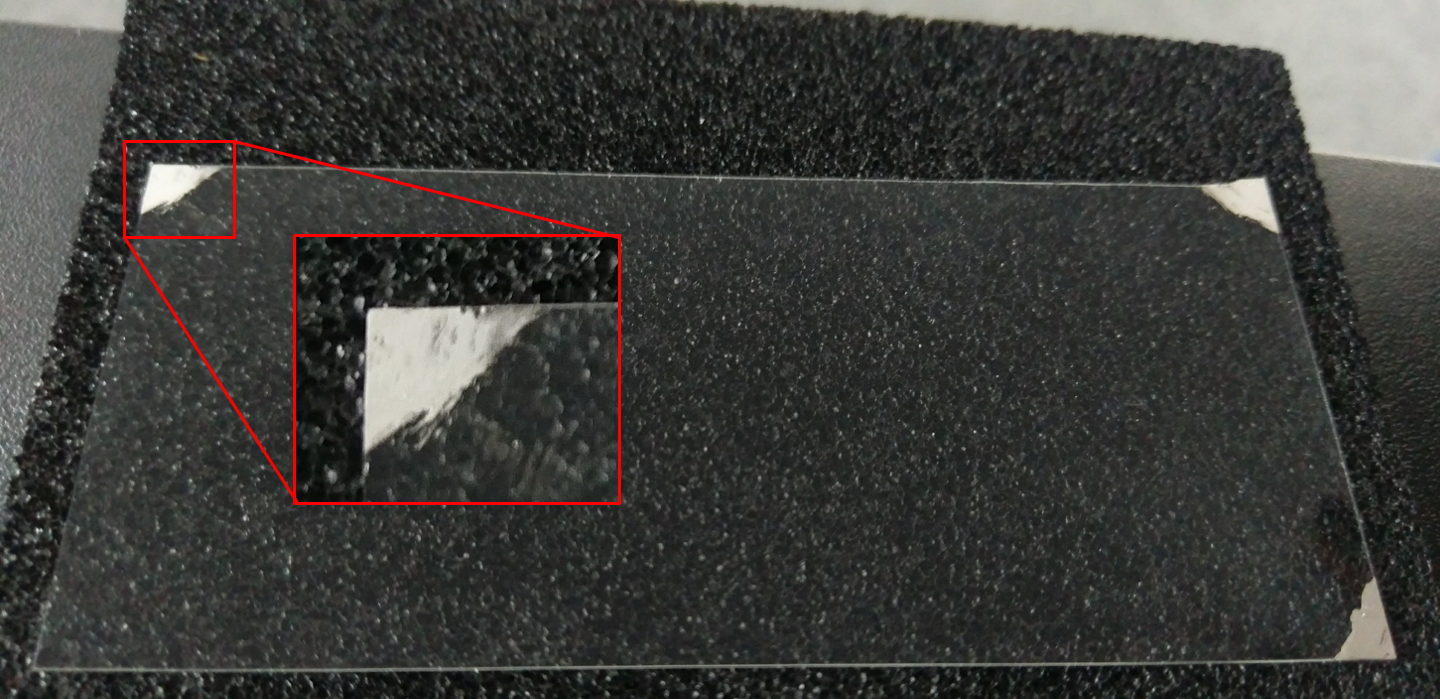
\includegraphics[width=0.8\linewidth]{Data/Precision_tests/Painted_corner.png}
\caption{Glass sample with silver painted corner.}
\label{fig:painted_corner}
\end{figure}

The step-by-step outline of this test is listed below:
\begin{enumerate}
\setlength\itemsep{-0.5em}
\item Move to the image acquiring position.
\item Acquire image and run pattern recognition.
\item Move aside for 5~mm in all three axes.
\item Move to the image acquiring position.
\item Acquire image and run pattern recognition.
\item Save data of the current iteration and go to the next one.
\end{enumerate}

After each step software saves the difference between measured coordinates before and after moving the arm with the camera. The distributions of these values are showed in Figure \ref{fig:corner_x}, Figure \ref{fig:corner_y} and Figure \ref{fig:corner_theta} for X-axis, Y-axis and theta, respectively. The test had 100~iterations done in a row.

\begin{figure}[ht]\centering
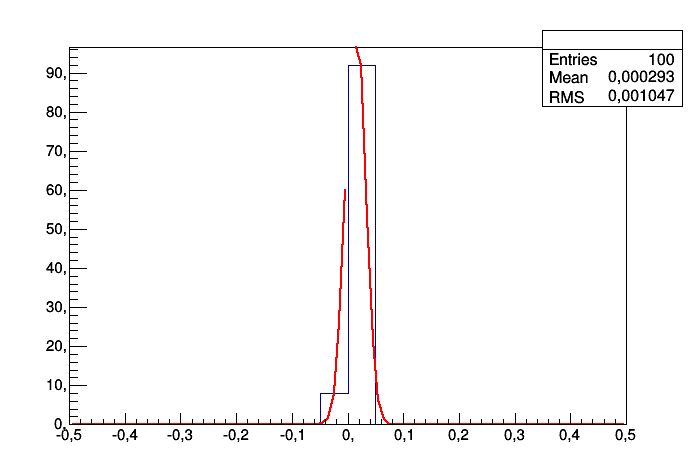
\includegraphics[width=0.8\linewidth]{Data/Precision_tests/Corner_c_x.png}
\caption{Distribution of the difference between detected X coordinate of the master image before and after moving the arm in each iteration. $\Delta X \approx 1~um$. }
\label{fig:corner_x}
\end{figure}

\begin{figure}[ht]\centering
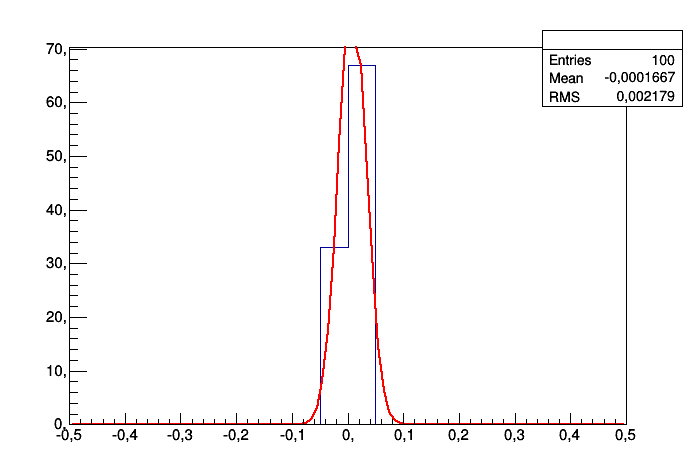
\includegraphics[width=0.8\linewidth]{Data/Precision_tests/Corner_c_y.png}
\caption{Distribution of the difference between detected Y coordinate of the master image before and after moving the arm in each iteration. $\Delta Y \approx 2~um$.}
\label{fig:corner_y}
\end{figure}

\begin{figure}[ht]\centering
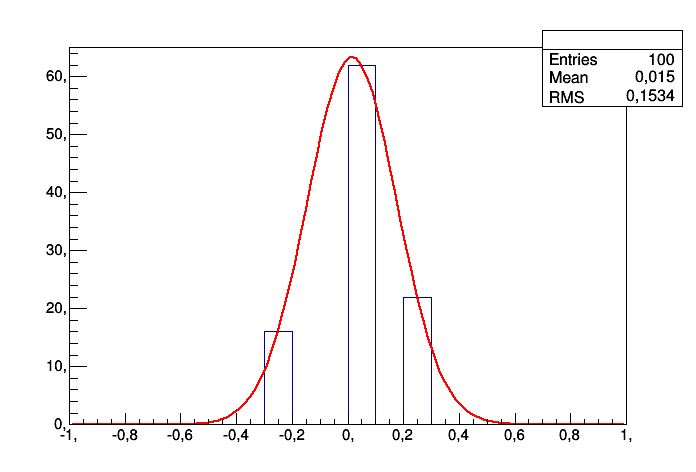
\includegraphics[width=0.8\linewidth]{Data/Precision_tests/Corner_c_theta.png}
\caption{Distribution of the difference between detected angle orientation of the master image relatively to the acquired image before and after moving the arm in each iteration. $\Delta theta \approx 0.15 ~degree$. }
\label{fig:corner_theta}
\end{figure}

Looking at the Figures \ref{fig:corner_x} and \ref{fig:corner_y} one can see that the X, Y detection of the pattern recognition has enough good precision (\underline{1-2~um of error [?]}), while the theta detection results do not look so precise. There are several reasons of such behaviour. The main one them is shown on the Figure \ref{fig:corner_threshold}.

Silver painted surface is not flat in 10~um scale. Due to this roughness different amount of light reflects to the camera from different points along the painted surface. That is why the painted corner contains various shades of grey, which in some points are darker, than the table underneath the sample (background). All these result into the picture one can see in the Figure \ref{fig:corner_threshold}. This kind of pictures has random distribution of dark areas on it. That is why the pattern recognition algorithm has such error while comparing two pictures (master template and acquired image) with random distribution of black areas. Moreover, this kind of tests lasts around one hour, which is long enough for the sun to change the ambient light in the laboratory. Even though all reasonably possible measures were done to prevent such effect, the acquired image is very sensitive for light. For example, the effect of the sun light can results in the threshold variation for 20 units (the color depth is 256) even with covered window in the laboratory.

\begin{figure}[ht]\centering
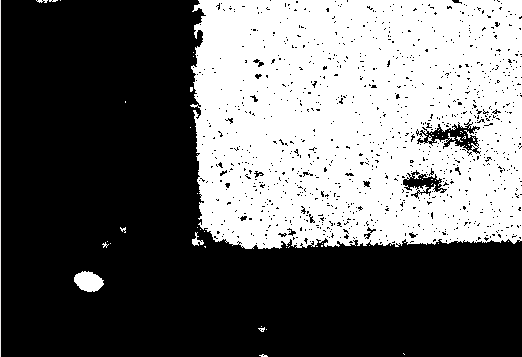
\includegraphics[width=0.8\linewidth]{Data/Precision_tests/Corner_thresholded.png}
\caption{The view of the corner after applying the Threshold.}
\label{fig:corner_threshold}
\end{figure}

\subsection{Pattern recognition on the marker of the dummy sensor}

The same test, but with dummy silicon sensor and real marker on it, was done. Before the test marker was aligned as much close to zero degrees as possible. At the Figure \ref{fig:thresholded_marker} one can see that the edge of the marker after applying Threshold is almost perfect (+/- one pixel). This fact itself is already a proof that Threshold step of pattern recognition is feasible.

\begin{figure}[ht]\centering
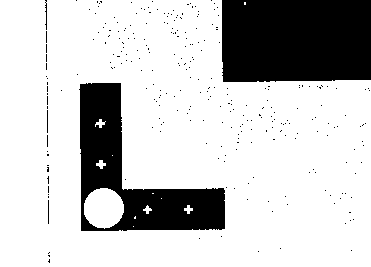
\includegraphics[width=0.6\linewidth]{Data/Precision_tests/Thresholded_marker.png}
\caption{Sensor marker after applying Threshold.}
\label{fig:thresholded_marker}
\end{figure}

The Distribution of X, Y coordinates and theta shows better results than with painted corner, which was expected. For X and Y it is less than a micron, which is already at the limit of camera resolution. $\Delta theta$ is one order of magnitude better than with painted corner --- $\approx 0.02  degree$.

A screenshot of the application during the test is shown on the Figure \ref{fig:zero_peak}. On the pattern recognition curve one can see that at 0 degree there is an unexpected short upward shot. This peak is not a fluctuation and it is not consist of only one point in the plot. As the scale increases, more points form this peak appear. It was not observed in the previous test just because the theta step was one order of magnitude bigger.

\begin{figure}[ht]\centering
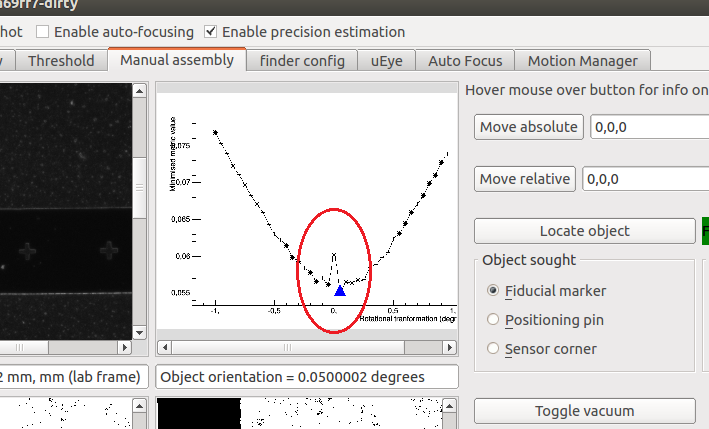
\includegraphics[width=0.8\linewidth]{Data/Precision_tests/Upward_shot.png}
\caption{Screenshot of application during precision estimation test with dummy silicon sensor and marker on it.}
\label{fig:zero_peak}
\end{figure}

\section{Pick-up and -down precision tests}

Next set of tests were oriented to explore the effect of picking-up/down on the precision of the system. In other words, will this process move the sample or not in XY plane. Due to the risk of breaking fragile silicon samples, we used glass ones.

\subsection{Pick-up and -down precision tests without assembly platform}

The first pick-up/down test was done without assembly platform. The step-by-step outline of this test is listed below:
\begin{enumerate}
\setlength\itemsep{-0.5em}
\item Move to the image acquiring position.
\item Acquire image and run pattern recognition.
\item Move to pre-pickup position.
\item Move to pickup position.
\item Turn negative vacuum on.
\item Move up.
\item Move down.
\item Release vacuum.
\item Move down.
\item Move to pre-pickup position.
\item Move to the image acquiring position.
\item Acquire image and run pattern recognition.
\item Save data of the current iteration and go to the next one.
\end{enumerate}

One can notice the step of moving first to pre-pickup position before going to the pick-up position and visa versa. This step is essential. The motion stage provides equal speed in all three axes, so when it receives a command to move to some position it starts to move with equal speed in each of three directions towards the destination simultaneously. As soon as destination in one axis is reached, it obviously stops moving in this axis while moving in other axes is going on. Therefore there is an unlike situation when the robotic arm reaches the sample in Z-axis while X and Y axes would still keep moving, which may cause damage or even break a sample. To prevent such situation we added the step of moving to pre-pickup position.

The results of the test showed movement of the sample, which could be noticed with a naked eye. In order to minimize this movement we decided to make a touch test -- the same as pick-up and -down, but without vacuum. Such kind of test can show the contribution of the touch to the sample movement in the pick-up and -down test. The results if this test was quite similar to the previous test, which means that the touch itself contributes the most to the sample movements in the pick-up and -down test. The interesting fact of this movement is its trend. On Figure \ref{fig:touch_move} one can see X and Y movement trends with respect to iteration number in the touch test. This plots show that the movement is not random and it is more or less constant both in value and direction.

\begin{figure}[ht]\centering
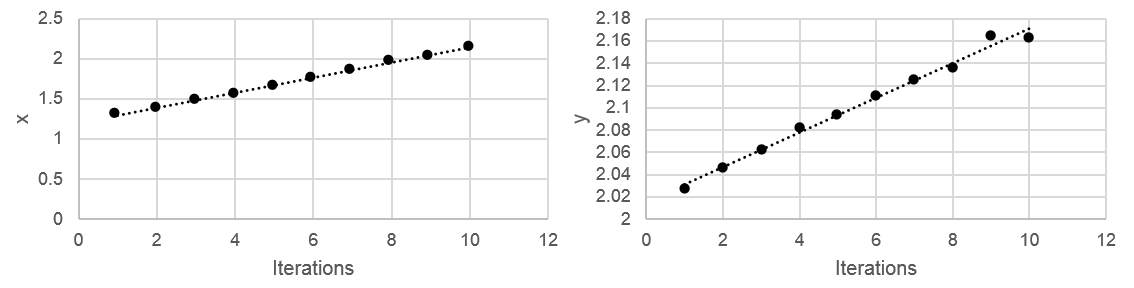
\includegraphics[width=1\linewidth]{Data/Precision_tests/XY_touch_movement.png}
\caption{X and Y movement trends with respect to iteration number in the touch test.}
\label{fig:touch_move}
\end{figure}

The most probable reason for such effect is that pick-up tool surface is not parallel to the table, where samples lay waiting for being picked-up. This fact perfectly corresponds to the constant movement of a sample to the one direction. Unfortunately, it is very complicated to align this surface parallel enough to make sample movement negligible. Another way to avoid this movement is to use an assembly platform, which can hold samples with vacuum underneath so they would be fixed.

\subsection{Pick-up and -down precision tests with assembly platform}

The step-by-step outline of the pick-up and -down test with the assembly platform is very similar to the one without it. The only difference is that samples are always fixed by the underneath vacuum and are only released, when the vacuum from pick-up tool is provided, so it can lift the sample upwards.

\begin{enumerate}
\setlength\itemsep{-0.5em}
\item Move to the image acquiring position.
\item Acquire image and run pattern recognition.
\item Move to pre-pickup position.
\item Move to pickup position.
\item Turn pick-up tool negative vacuum on.
\item Turn assembly platform negative vacuum off.
\item Move up.
\item Move down.
\item Turn assembly platform negative vacuum on.
\item Turn pick-up tool negative vacuum off.
\item Move down.
\item Move to pre-pickup position.
\item Move to the image acquiring position.
\item Acquire image and run pattern recognition.
\item Save data of the current iteration and go to the next one.
\end{enumerate}

Distribution of the difference between detected X coordinate of the master image before and after moving the arm in each iteration is shown on the Figure \ref{fig:platform_distribution}.

\begin{figure}[ht]\centering
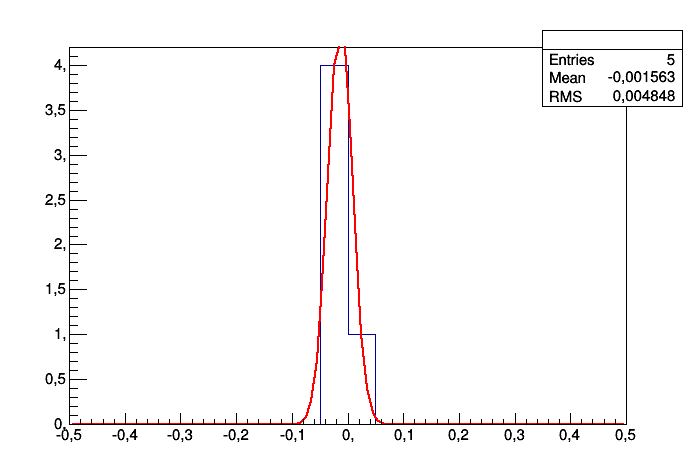
\includegraphics[width=0.8\linewidth]{Data/Precision_tests/Platform_x_distrib.png}
\caption{Distribution of the difference between detected X coordinate of the master image before and after moving the arm in each iteration. $\Delta X \approx 4~um$. }
\label{fig:platform_distribution}
\end{figure}

As one can see from the Figure \ref{fig:platform_distribution}, $\Delta X \approx 4~um$, which is very close to the limit of 1~um of the pattern recognition itself without touching the sample. Moreover, the X and Y coordinates show no trend with respect to the iteration number. Taking into account these results, it is possible to say that using an assembly platform can fix samples enough tight, so it is possible to neglect their movements.

\section{First assembled prototype}

After all tests mentioned above it was possible to assemble the very first prototype of the module. To test the precision of the assembling module for the first time it was decided to use simplified assembly algorithm, which would provide maximum precision only on one corner. Schematic view of the first module prototype is shown on the Figure \ref{fig:module_prototype}.

\begin{figure}[ht]\centering
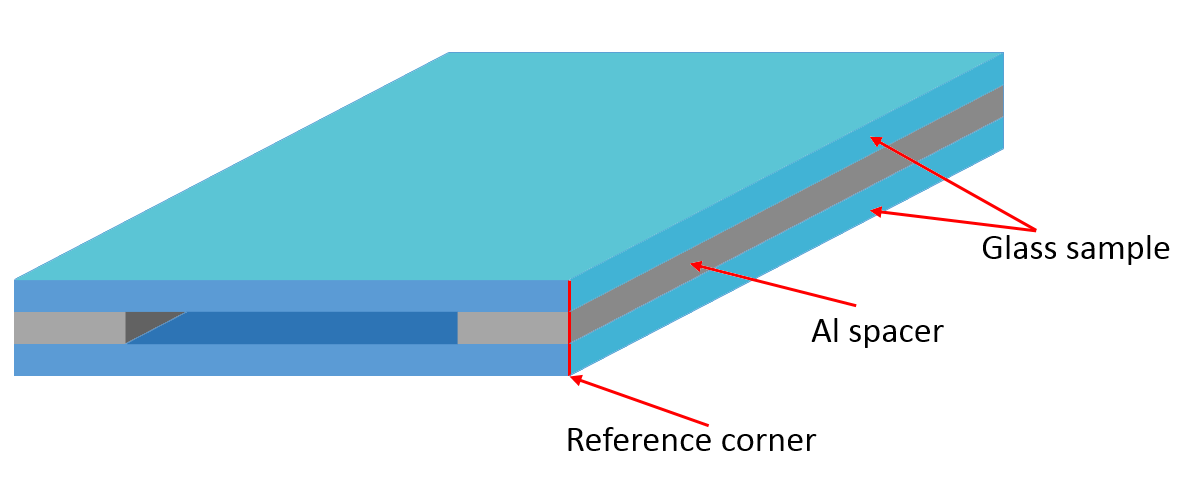
\includegraphics[width=0.8\linewidth]{Data/Precision_tests/Module_prototype.png}
\caption{Schematic view of the first module prototype.}
\label{fig:module_prototype}
\end{figure}

The step-by-step outline of the assembly process is listed below:

\begin{enumerate}
\setlength\itemsep{-0.5em}
\item \textit{Place and align top sample parallel to X-axis of motion stage and lift it up with pick-up tool.} Place top sample on the assembly platform and fix it with vacuum. Find with the pattern recognition its orientation in space. Rotate the platform to align top sample parallel to the edge of the pick up tool. As soon as theta recognition do not provide enough accuracy, the following method was used. Move camera for 5~cm along the sample edge and measure the shift of the sample edge. Knowing two cathetus of it is possible to find the angle of the right triangle, which equals to the angle between sample edge and x-axis of motion stage. Rotate the assembly platform for this angle. To sum-up, first -- rough top sample orientation estimation with direct pattern recognition, second -- precise calculated sample orientation with Pythagorean theorem. Now the top sample is aligned enough parallel to the X-axis of the motion stage. Next, save position of the reference corner with a pattern recognition. Finally, pick-up top sample with pick-up tool and leave it there.
\item \textit{Place Al spacers.} Put Al spacers to the inserts, fix them with bottom vacuum and align them parallel to the X-axis of the motion stage. Absolutely the same way as with top sample. Save the coordination of the reference corner with pattern recognition. Comparing coordinates of the reference corners of Al spacer and top sample, move the robotic arm in XY plane of the motion stage so they would match.
\item \textit{Glue Al spacers to the top sample.} Place the glue on Al spacers and move robotic arm with attached top sample down. It is important to move robotic arm down for exactly correct distance. This topic was discussed in details in the Module Assembly Chapter. Wait glue to be cured and lift glued structure (Al spacers and top sample) from assembly platform.
\item \textit{Place and align bottom sample parallel to X-axis of motion stage.} Place bottom sample on the assembly platform and fix it with bottom vacuum. Make the parallel alignment to the X-axis with the same method as with top sample. Find XY coordinates of the reference corner with the pattern recognition. Compare them to XY coordinates of spacers and top sample. Move the robotic arm with attached structure glued before to match reference corners of all parts of the module.
\item \textit{Final gluing.} Put the glue on the bottom sample and move robotic arm down for correct distance to glue entire prototype. After glue is cured the assembly process is finished.
\end{enumerate}

The glued prototype is shown on Figure \ref{fig:module_prototype}.

\begin{figure}[ht]\centering
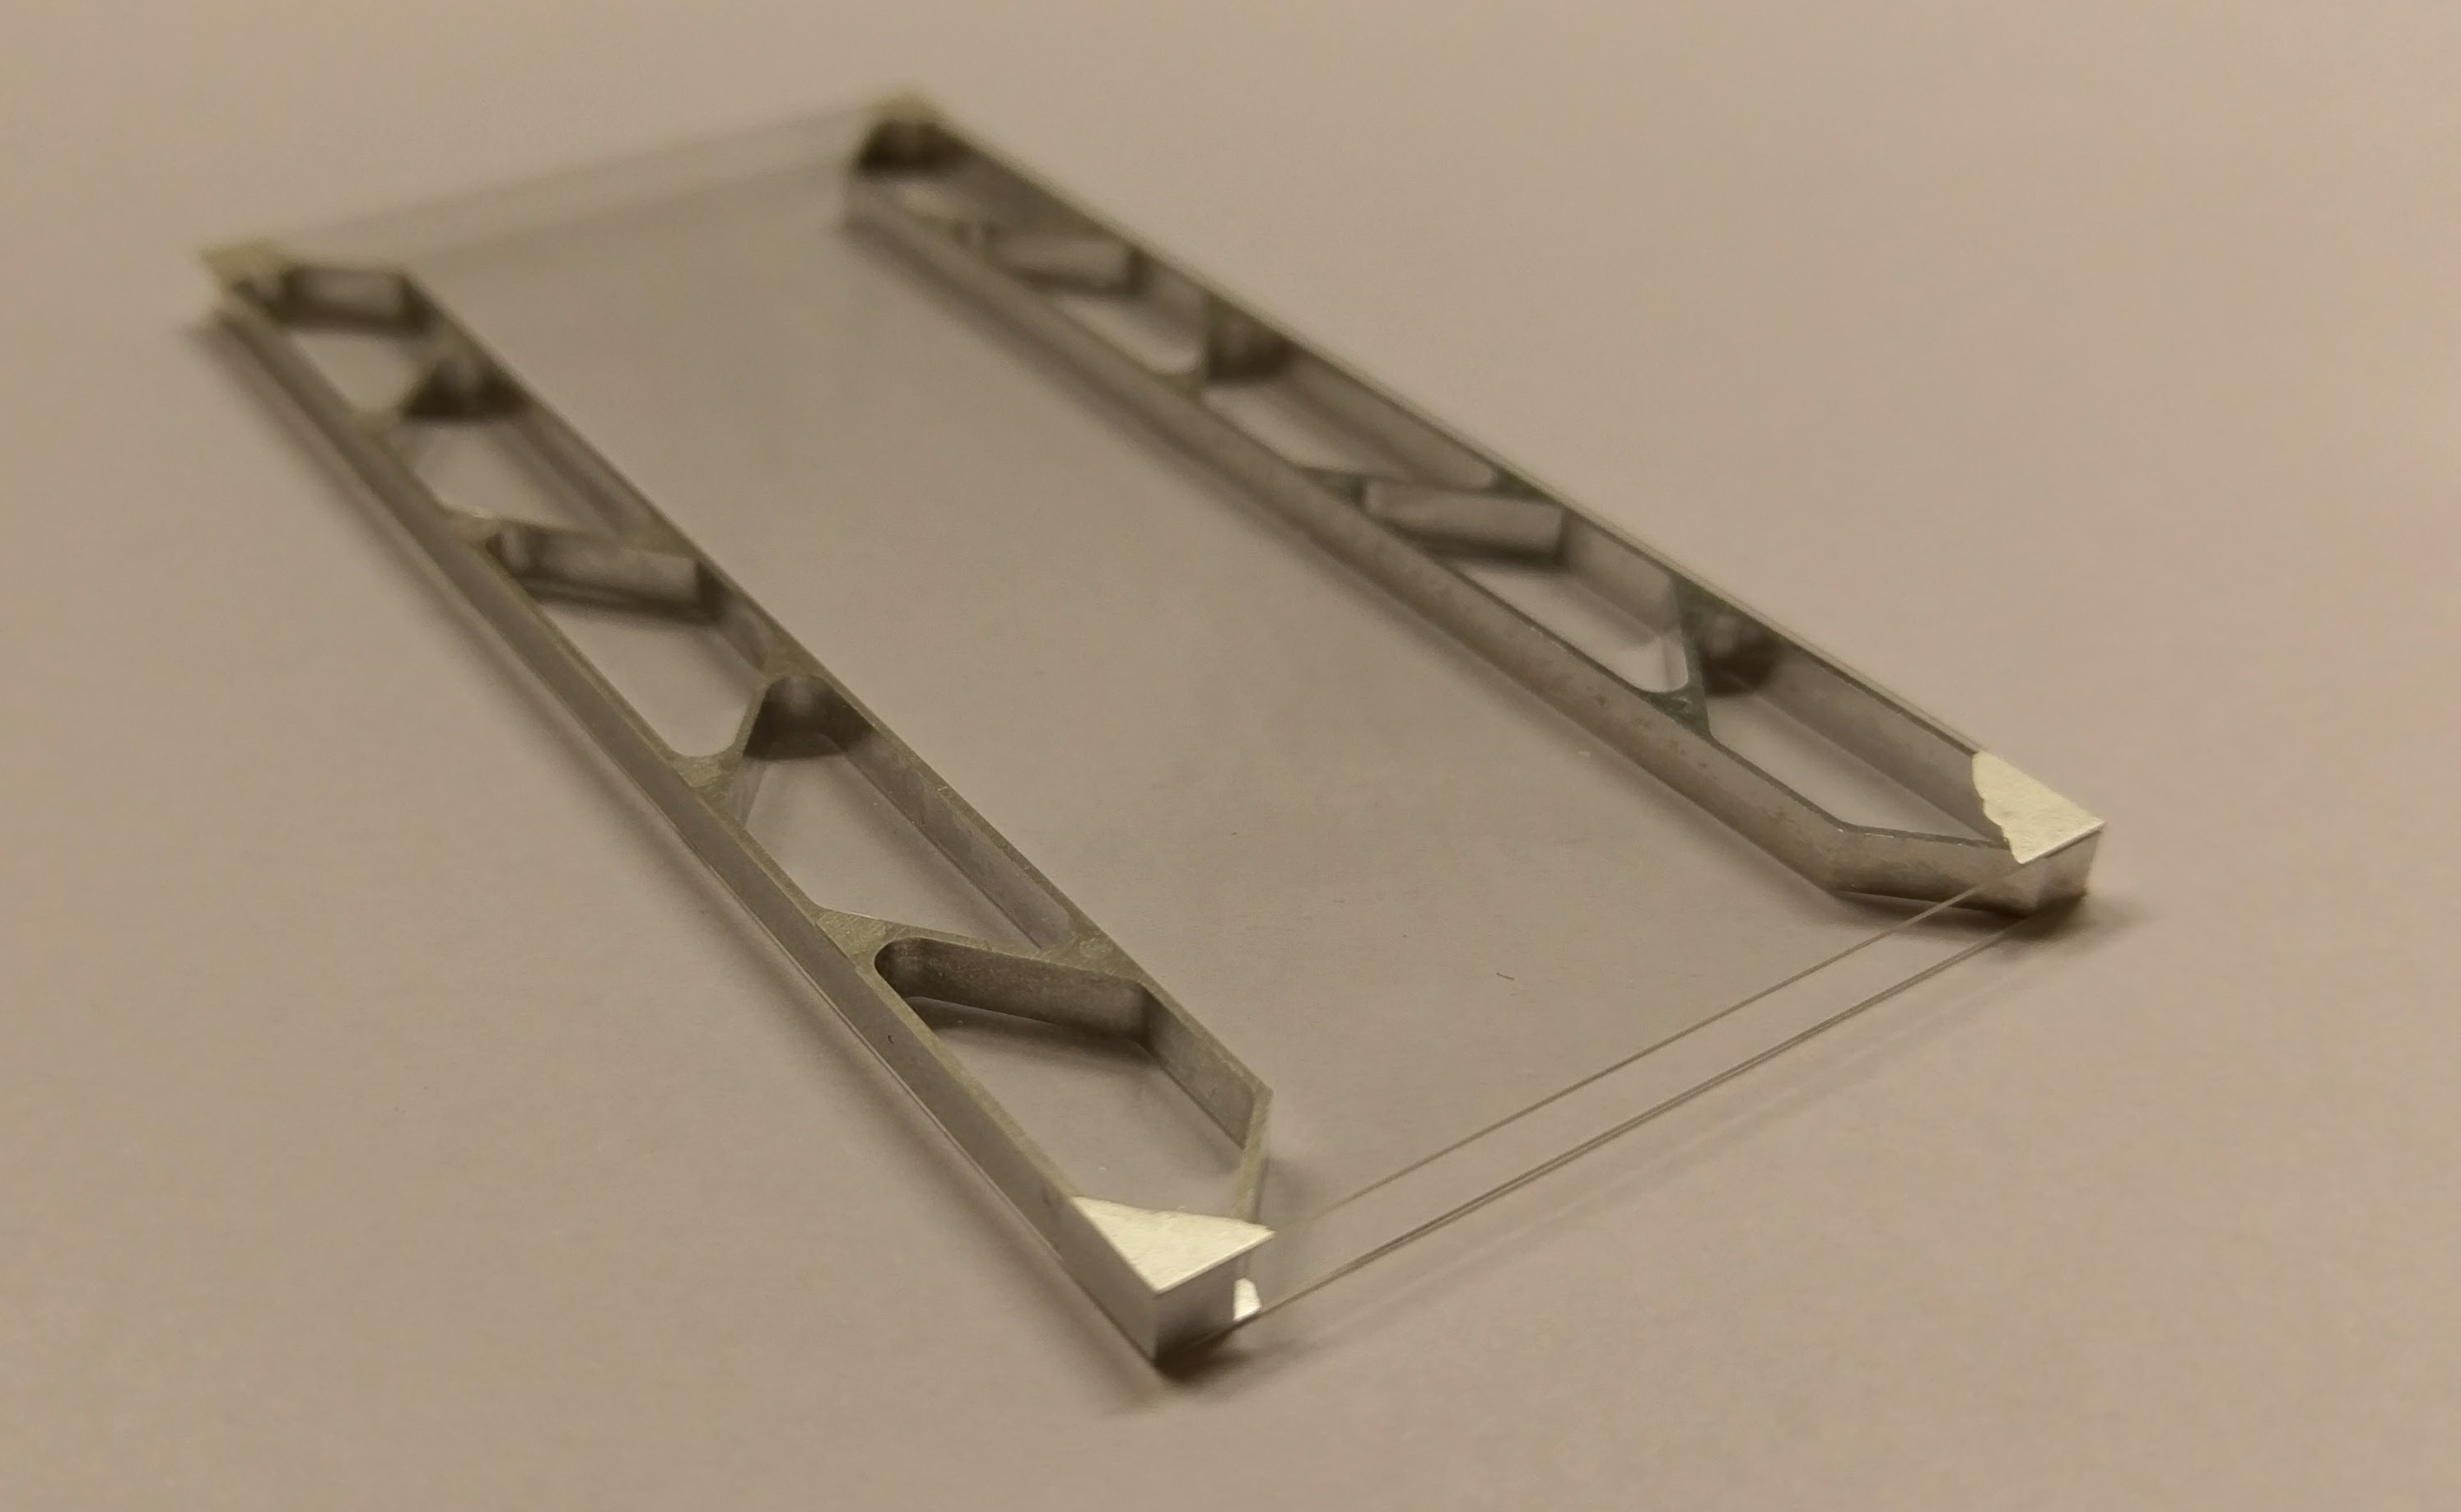
\includegraphics[width=1\linewidth]{Data/Precision_tests/Prototype_photo.png}
\caption{Photo of the first assembled prototype.}
\label{fig:module_prototype}
\end{figure}

We used simplified algorithm for the first prototype assembly aligning only one corner. The quality of assembled prototype is very promising. It meet all necessary requirements. On the Figure \ref{fig:prototype_macro} one can see the photo of the reference corner from the microscope. Pictures form other directions look very similar having approximately the same accuracy.

\begin{figure}[ht]\centering
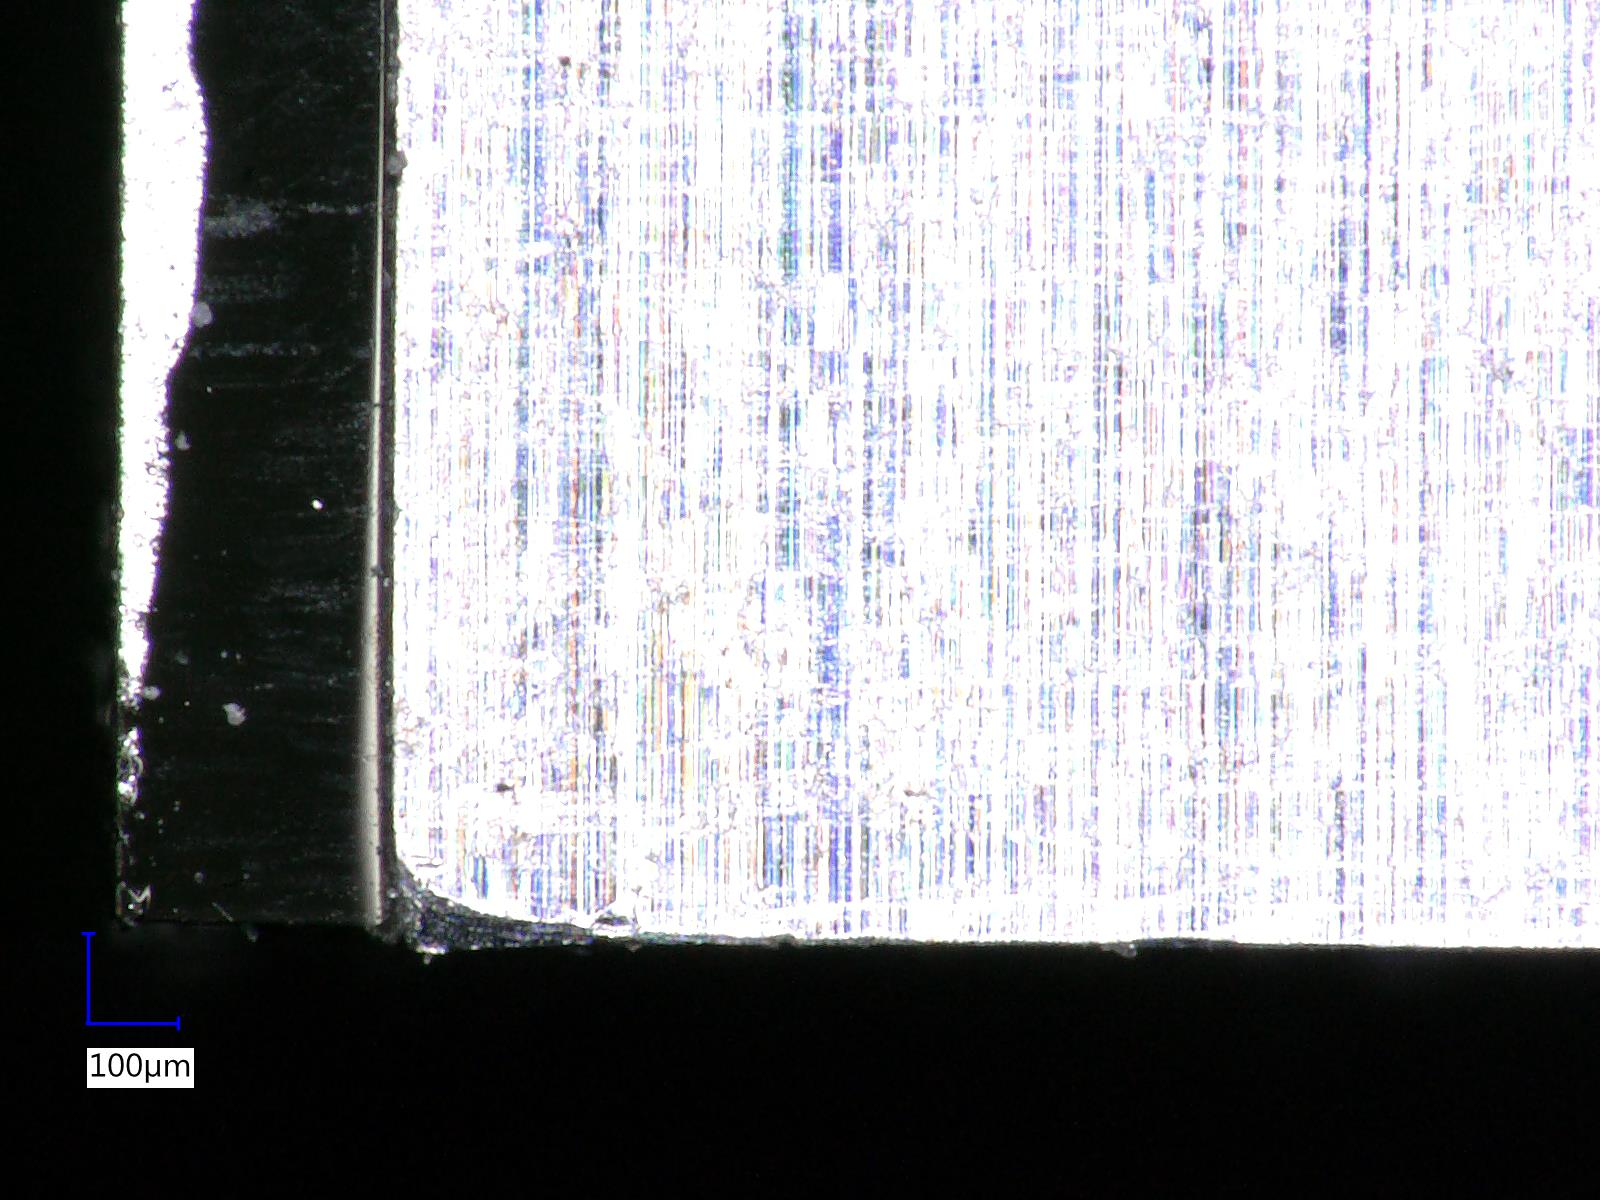
\includegraphics[width=1\linewidth]{Data/Precision_tests/Top_sensor_X_view.png}
\caption{Microscope photo of the reference corner of the first prototype. Misalignment of the components is around 20~um.}
\label{fig:prototype_macro}
\end{figure}

This assembled prototype proved the feasibility of the automated assembly and showed lots of issues to be solved in future. Even though it has only silver pained corner, not precise lithography, this prototype showed very good results in terms of assembling accuracy.
